% Chapter 2

\chapter{The LHC and CMS experiment} % 
\label{cha:detector}
\section{The Large Hadron Collider}
\label{lhc_intro}
%LHC intro 
The LHC is a 27km circular circumference storage ring, accelerator and collider for 
both protons and Pb ions. It is situated in a stable environment in a tunnel 
100 metres underneath the Franco-Swiss border near Geneva, Switzerland.
A double-ring synchotron, it is designed to collide proton-proton (pp)
pairs with a centre of mass energy of up to $\sqrt{s}=14\TeV$ and a 
luminosity of up to $10^{34}\cm^{-2}s^{-1}$. This makes the LHC the only collider
in operation able to directly probe $\TeV$ scale physics. 

The injected beams in the LHC are accelerated and stored for each physics run using 
a 400 MHz superconducting cavity system. The beams of protons or pB ions 
are merged at four sections around the ring to enable collisions at interaction points.
At each of these four interaction points lies one of the four main 
experiments at the LHC; A Large Ion Collider Experiment (ALICE)~\cite{ALICE},
A Toroidal LHC Apparatus (ATLAS)~\cite{ATLAS}, the Compact Muon Solenoid (CMS)~\cite{CMS}
and Large Hadron Collider Beauty (LHCb)~\cite{LHCb} which record the collisions. Figure~\ref{fig:LHC-diagram} shows the layout of the LHC ring including
the positions of the four main detectors. The proton beams are made up of many `bunches' of approximately $1.1\times10^{11}$
protons localised into less than 1 ns (or 30$\cm$) in the direction of motion.
The beams are formed inside the Proton Synchrotron (PS) from bunches of protons 25 ns apart with an energy of 26 \GeV. 
The protons are then accelerated in the Super Proton Synchrotron (SPS) to 450 \GeV~before being injected into the LHC at
the points shown in Figure~\ref{fig:LHC-diagram}. Once injected into the LHC, radio frequency (RF) cavities 
provide around 275kW of RF power independently to each beam to accelerate the protons
to half the operating centre of mass energy for collisions.
The LHC operates as a storage ring for the accelerated beams using 1232 
superconducting dipole magnets in the eight arc segments. These provide magnetic fields of up to $8T$ to steer the beams. 
High precision quadropole and higher order magnets at the interaction points are used to position and focus the beams to 
maximise the occurrence of high momentum collisions and therefore the luminosity. The average number of simultaneous collisions
per bunch crossing, in time pileup (PU), for the work in this thesis was $\approx25$.
The luminosity in the LHC is not constant over a physics run, but decays due to the degradation 
of intensities and emittance of the circulating beams (mainly due to loss from collisions). Eventually,
the beam is dumped and the acceleration process is started again. An efficient turn around between
dumping the beam and the start of a new physics run of 
around 6 hours allows the luminosity collected by CMS to be maximised. 

\begin{figure}
\centering
    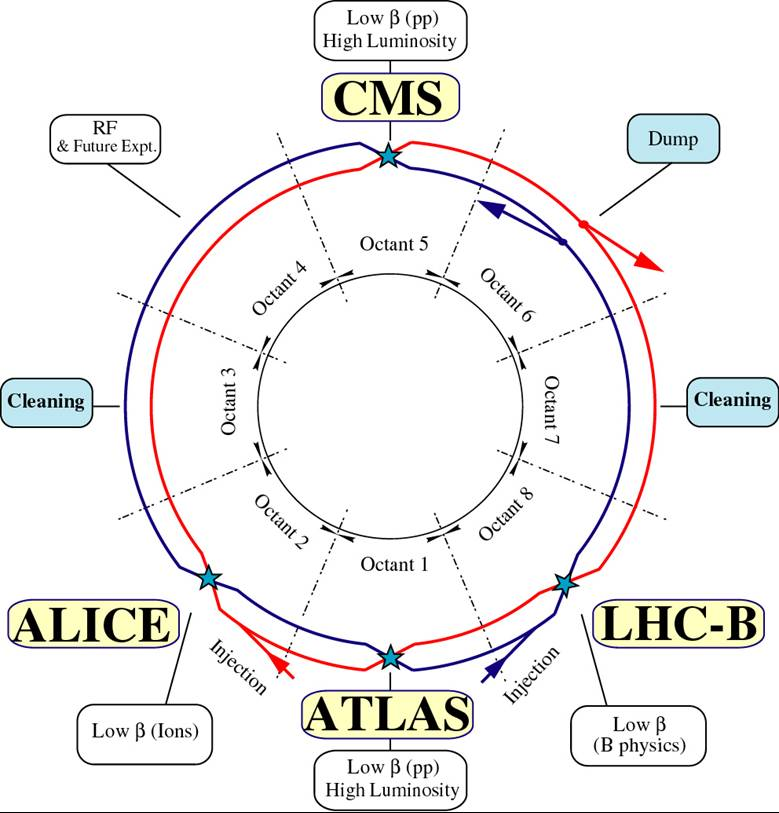
\includegraphics[width=0.6\textwidth]{./Figures/detector/lhcDiagram}
  \caption{Schematic layout of the LHC showing the position of the four main detectors as
  well as the RF systems.}
  \label{fig:LHC-diagram}
\end{figure}

\subsection{LHC run conditions}

The first physics runs of the LHC from 2010 to 2013 (Run 1) reached energies of 3.5 and 4\TeV~per beam and 
provided record-breaking integrated luminosities. The data collected allowed the 
discovery of the Higgs boson~\cite{cmsHiggs,atlasHiggs} as well as enabling many new regions of parameter space
to be probed. From 2013 to mid-2015 (Long Shutdown 1) the LHC was shut down for upgrade to allow design
energies to be reached. All magnet interconnectors were inspected and replaced, where necessary,
and the dipole magnets underwent a quench training programme. 

From 2015 to 2016 (Run 2, which will continue up to 2018) the LHC has been running with record beam energies 
of $6.5 \TeV$ per beam with bunch spacings of 25 and 50 ns. 
As shown in Figure~\ref{fig:LHC-integrated-lumi}, by July 2016, $16.0 \ifb$ of integrated luminosity was
delivered to the CMS and ATLAS detectors, with $13.8 \ifb$ recorded by CMS. The dataset is validated 
to ensure the exclusion of runs in which the data quality may be affected by detector subsystem. 
The luminosity of this `certified' dataset is $12.9 \ifb$ and it is this dataset, 
at a centre of mass energy of $\sqrt{s} = 13 \TeV$, which forms the basis for the work in this thesis.

%%%FIGURE - LHC lumi plot
\begin{figure}
\centering
    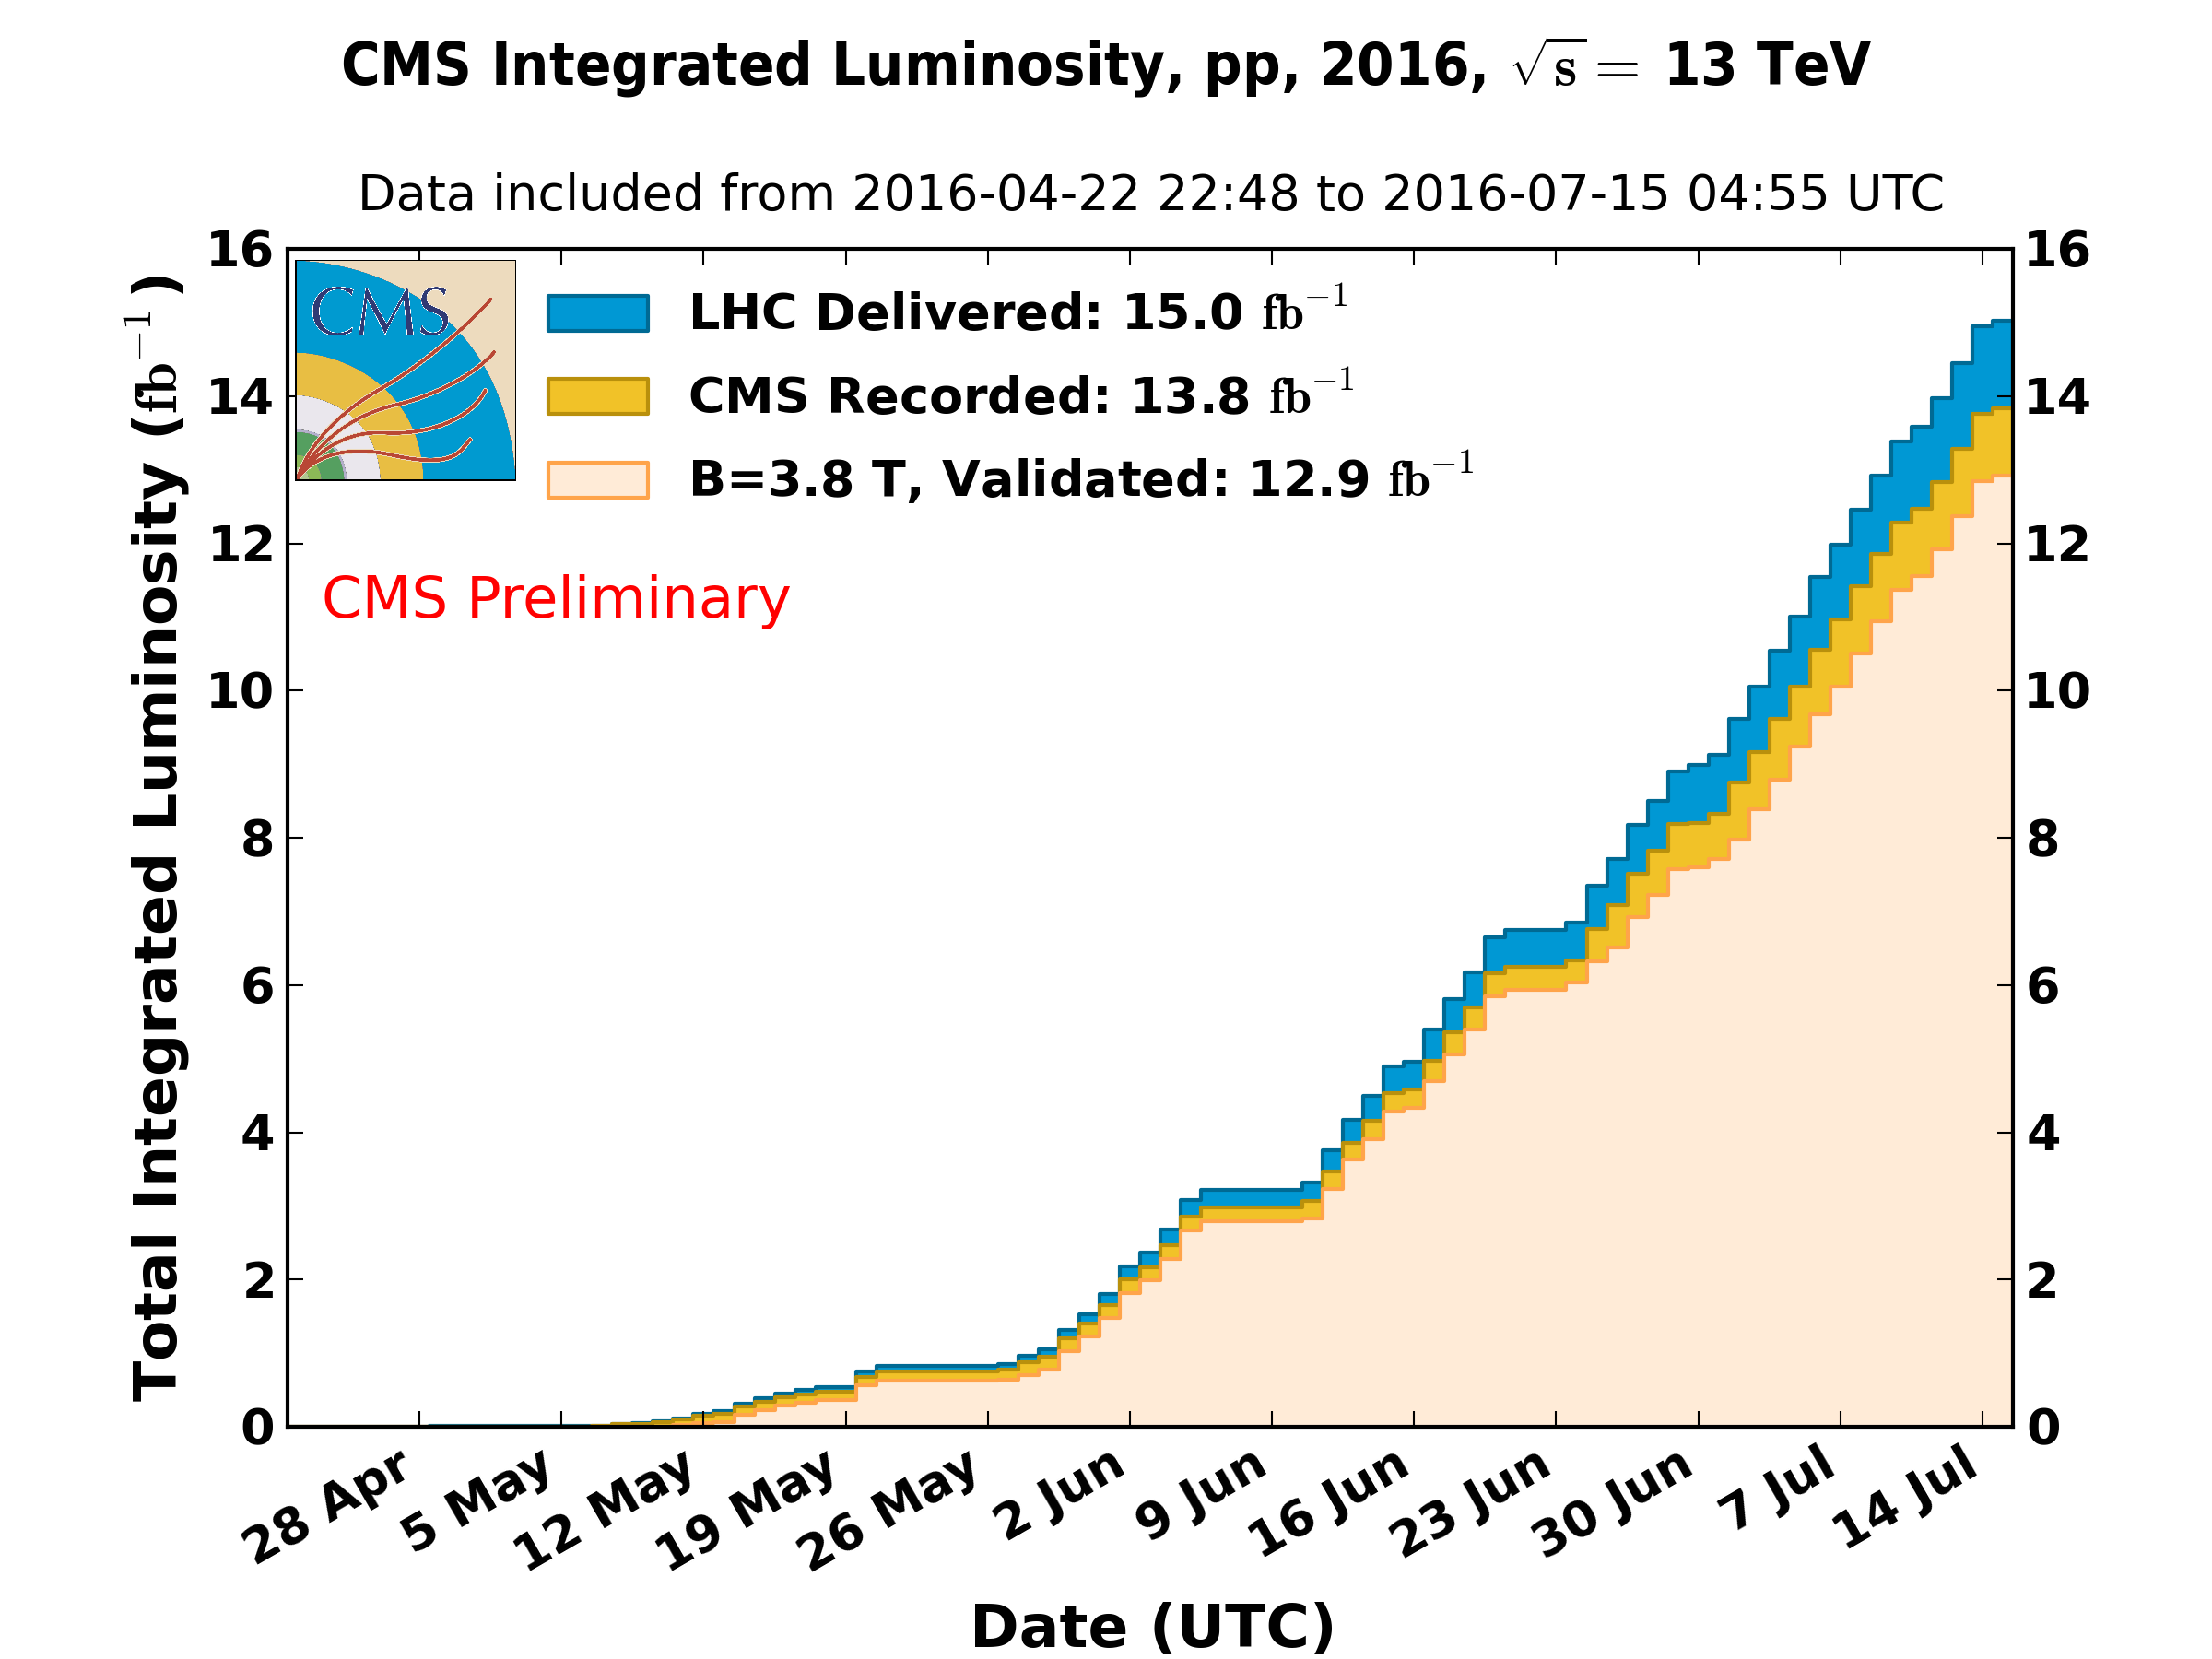
\includegraphics[width=0.6\textwidth]{./Figures/detector/int_lumi_per_day_cumulative_pp_2016_Golden_ICHEP}
  \caption{Integrated luminosity measured online versus day delivered to CMS (blue)
  and recorded by CMS (orange) during stable beams for p-p collisions at $\sqrt{s} = 13 \TeV$~\cite{cmslumi}.}
  \label{fig:LHC-integrated-lumi}
\end{figure}

%----------------------------------------------------------------------------------------
\section{The CMS detector}
The Compact Muon Solenoid (CMS~\cite{CMS}) is one of two general-purpose detectors at the LHC 
which have performed exceptionally well during the physics runs of the LHC. The main design goals
for CMS were to discover the Higgs boson as well as to search for generic models 
of new physics. To achieve this, CMS provides efficient identification and measurement
of physics objects including muons, electrons, photons, taus and hadronic showers over a
wide range of momenta and energies. Each major subsystem is made of a barrel
and two endcaps to give coverage of almost $4\pi$ in solid angle. 
This barrel design ensures global momentum imbalance can be effectively 
reconstructed, allowing the missing energy predicted in many new models of physics to be
precisely measured. A more detailed description may be found in~\cite{CMS}.  

The coordinate system used by CMS takes the origin at 
the collision point. The z-axis points along the beam direction while the x-axis points radially inward
towards the centre of the LHC and the y-axis points vertically upward.
The polar angle, $\theta$, is measured from the z-axis and defines the pseudorapidity, $\eta=-ln(tan(\theta/2))$. 
This is used in preference to $\theta$ as the difference between the pseudorapidity of two 
particles is invariant under boosts along the z-axis~\cite{cms_iop}. 
The $\eta$ coverage of CMS is $|\eta|<5$. The azimuthal angle, $\phi$, is defined from the x-axis in the x-y plane.
This allows the definition of $\Delta R = \sqrt{(\Delta\phi^2+\Delta\eta^2)}$, commonly used to measure the 
angular difference between objects. Transverse energies and momenta, $E_T $ and $p_T$ respectively, are defined 
as $E_T = E\sin(\theta)$ and $p_T = \sqrt{(p_{x}^2+p_{y}^2)}$. Momentum imbalances are measured as the negative 
vector sums of the momenta of the relevant objects in the x-y plane. 

\begin{figure}
\centering
    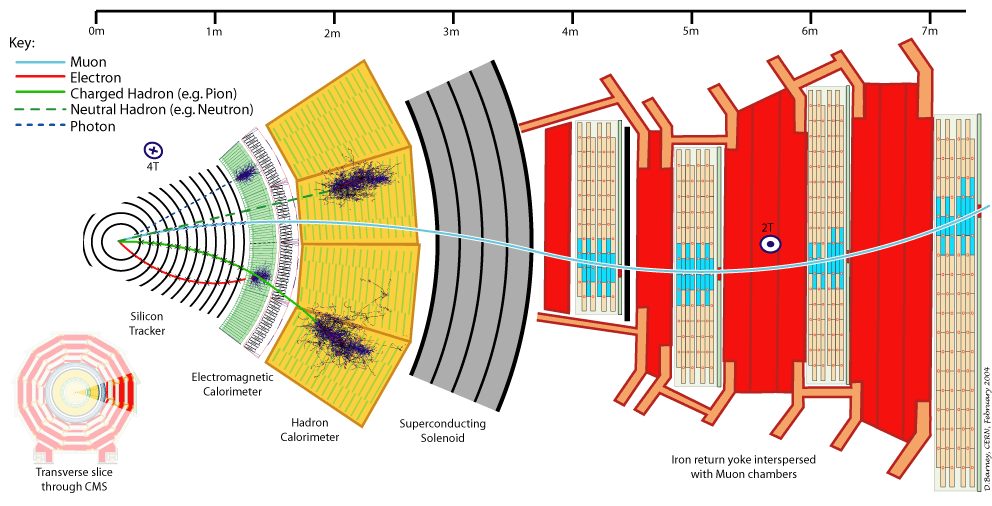
\includegraphics[width=0.6\textwidth]{./Figures/detector/CMS_Slice.jpg}
  \caption{Cross section of CMS showing the paths of various particle types 
  through different segments of the detector~\cite{cmsslice}}
  \label{CMS_SLICE}
\end{figure}

Figure \ref{CMS_SLICE} shows a cross section of CMS in the x-y plane as well as introducing the major detector components that will be described 
in detail in this section. The tracker lies closest to the beam and, as for the calorimetry subsystems, is situated within a magnetic field of 3.8T provided
by the superconducting solenoid. It measures the curved trajectory of charged particles through this magnetic field to determine their momenta 
as well as the location of primary and secondary vertices. The tracker is followed by the Electromagnetic Calorimeter (ECAL),
which measures energy deposited in electromagnetic showers from particles such as electrons and photons and is separated in barrel and endcap 
components for the central and forward regions respectively. The Hadronic Calorimeter (HCAL) lies outside the 
ECAL and measures energy from nuclear interactions of hadronic particles. It is a sampling calorimeter
made up of several layers of absorber and scintillator to allow hadron showers to be measured over a maximum of around 11 radiation lengths. 
The coverage of the hadron calorimeter is extended into the forward regions with the Hadronic Forward calorimeter (HF). Enclosing the calorimetry and tracking subsystems 
is the superconducting solenoid which generates the magnetic field. Outside the solenoid, the iron return yoke lies interspersed with muon chambers, forming the outermost components of the detector. 
Muons are minimally ionising particles (MIPs), depositing little energy within the detector, and typically reach the cavern containing the detector. 
The barrel muon system is composed of drift-tubes (DT) and resistive plate chambers (RPC). These provide
high resolution hit timing and positioning to determine the muon trajectory. In the forward region the DTs are 
replaced by cathode strip chambers (CSC) which have greater resistance to the higher 
radiation flux occurring along the beamline. 

\section{Tracker}
The CMS tracker is an all-silicon tracker with an area sensitive to charged particles of around 200 $m^2$. It is designed to measure hits along the
curved trajectories of charged particles that result from the high energy p-p collisions. A cross section of the tracker in the $r$-$z$ plane is shown in Fig~\ref{TRACKER_SLICE}.
The tracker has coverage for $|\eta| < 2.5$ and achieves an optimal efficiency in the barrel region $|\eta| < 0.9$~\cite{tracker_performance,tracker_tdr}. 
Close to the interaction vertex, $r < 20\cm$, where the particle flux is maximal ($~10^7/s$), is the pixel detector. This system consists of an inner region of 66 million silicon 
pixels of $100\mum \times 150\mum$ in three overlapping layers and a forward region with two endcap discs on each side.
For $r > 20\cm$ the particle flux drops to enable the use of larger silicon microstrips. These range in size from at least $10 \cm \times 80 \mum$ for the 
tracker inner barrel (TIB) region 
at intermediate values of $r$ ($20\cm < r < 55\cm$) to at least $25\cm \times 180\mum$ for the outer barrel (TOB) region ($55 \cm < r < 110 \cm$). The forward region
for $r > 20\cm$ is covered by endcap disks divided into the 9 disks of the tracker end cap (TEC) for the $120 \cm < |z| < 280 \cm$ region and 
3 tracker inner discs (TID) lying between the TIB and TEC. The TID and first 3 disks of the TEC have sensors of thickness $320\mum$ while the remainder of the TEC disks
have sensors of thickness $500\mum$~\cite{tracker_tdr}.

\begin{figure}
\centering
    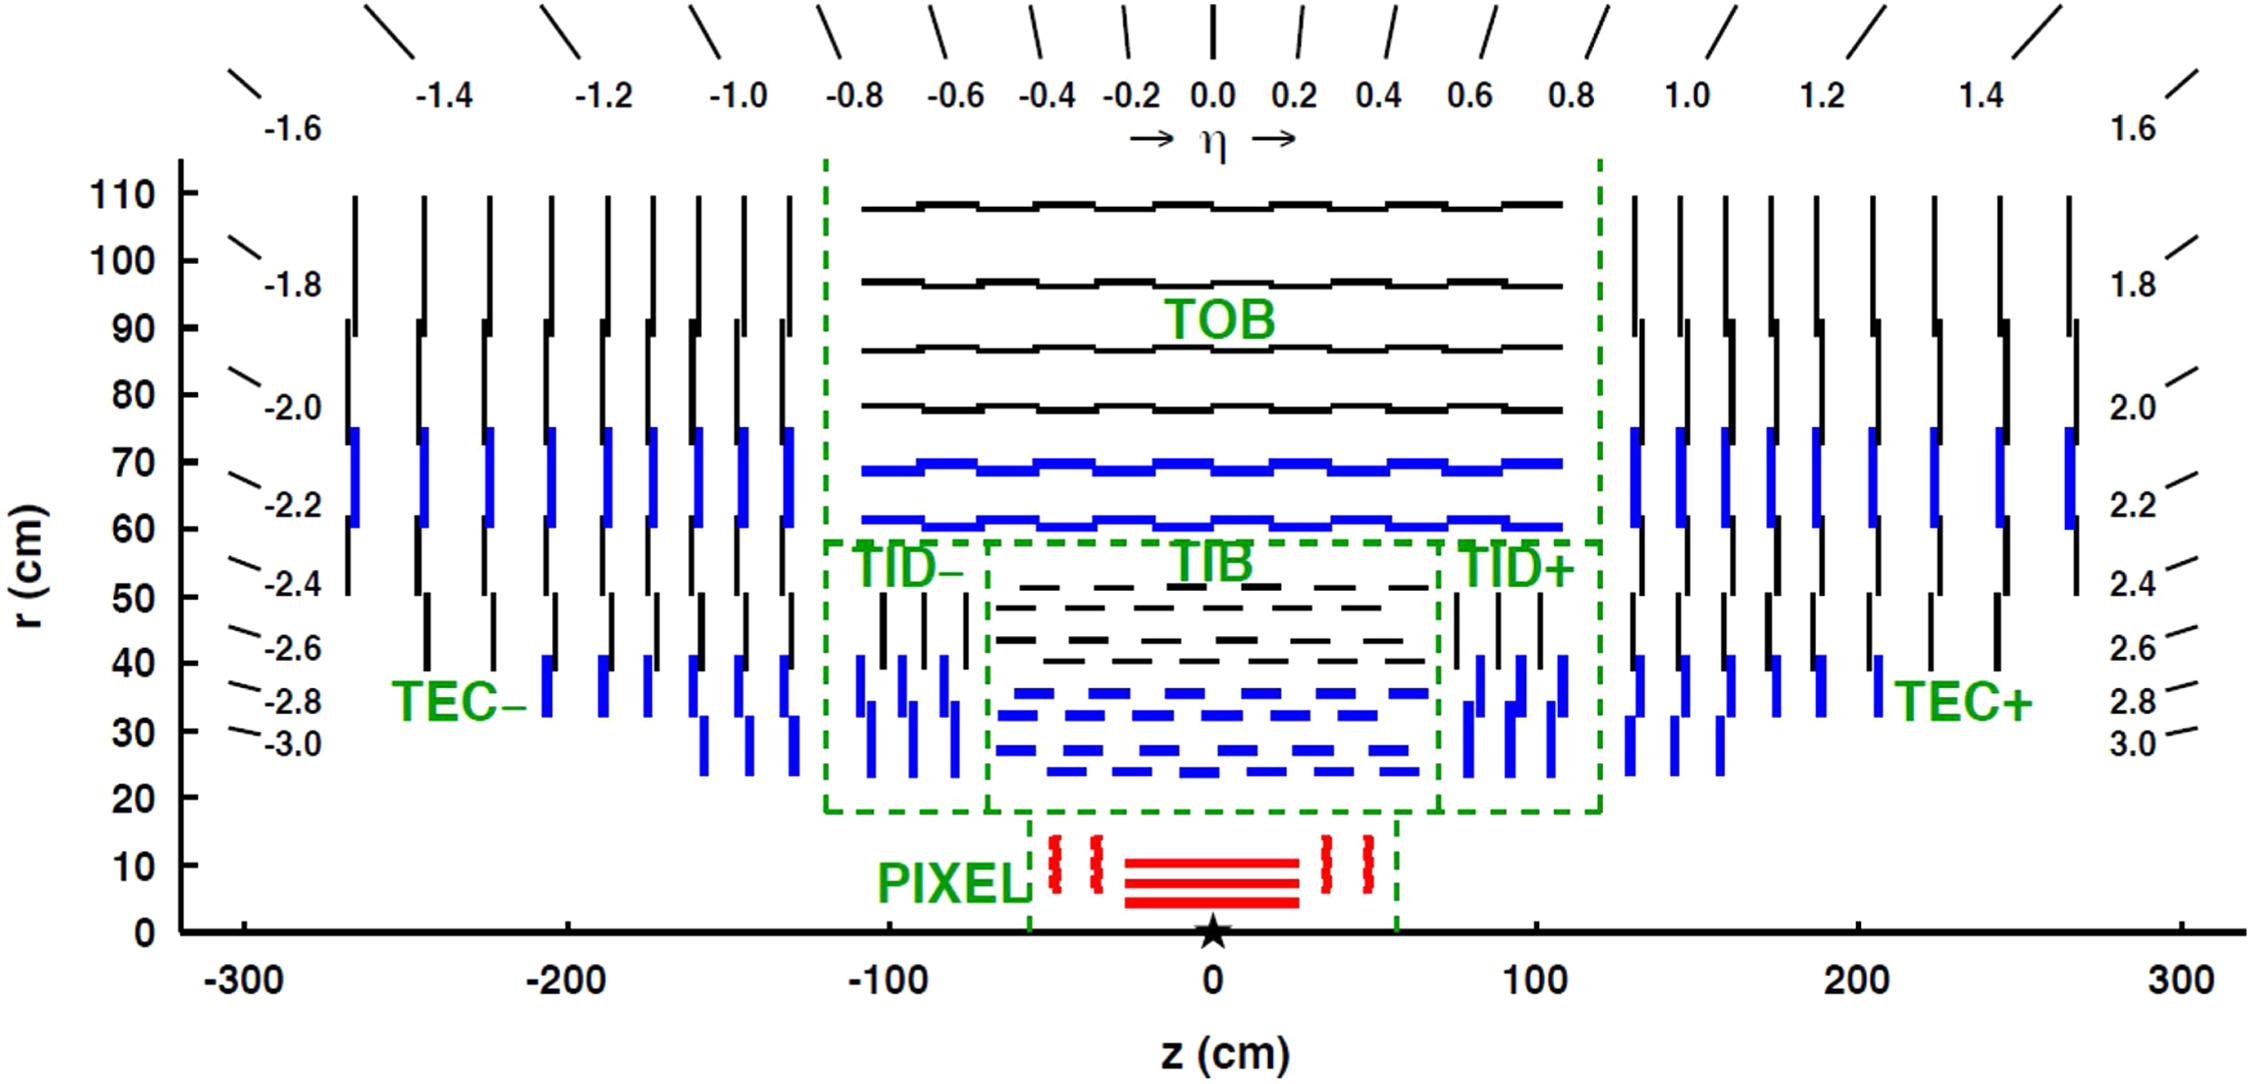
\includegraphics[width=0.6\textwidth]{./Figures/detector/CMS2Dtracker}
  \caption{A quarter cross section of the CMS tracker showing the pixel and strip~components~\cite{tracker_fig}}
  \label{TRACKER_SLICE}
\end{figure}

To measure the trajectories the tracker must effectively detect hits from charged particles. The efficiency for the 
hit reconstruction, defined as the fraction of particles with $p_T > 1 GeV$ passing through the fiducial regions of the sensors
in a layer for which hits are recorded, ranges from 99\% in the strip detector to 99.5\% for the pixel detector.
The position resolution for the hits also determines the track finding performance; for
the pixel detector the resolution in the $r$-$\phi$ plane is $\sim10\mum$ and $\sim20-40\mum$ along
the $z$ direction while the $r$-$\phi$ resolution for the strip detector ranges from $\sim13-47\mum$.

\section{Electromagnetic calorimeter}

The high precision measurement of the energy and position of electrons and photons resulting from 
processes such as Higgs decay is an important design goal of the CMS experiment. Additionally,
a substantial energy fraction of jets, which are central to the analysis outlined in this
thesis, is formed of photons whose properties cannot be measured in any other subsystem.

The CMS ECAL is formed of high density lead tungstate ($PbWO_4$) crystals incorporating an ECAL barrel section (EB) 
and two ECAL endcaps (EE) outside the tracker~\cite{ecal_tdr}. The high density (8.28$g/\cm^3$), short radiation length (0.89$\cm$) 
and small Moliere radius (2.2$\cm$) of the crystal are optimal for a compact calorimeter with high granularity. In addition the 
crystals are radiation hard (up to 10 Mrad) and have a fast scintillation decay time (80\% of the light is emitted within $25ns$)
comparable to the smallest bunch spacing provided by the LHC. 

The EB has an inner radius of 129$\cm$ and covers the range $|\eta| < 1.479$. The crystals are arranged into 36 
identical `supermodules' which surround the beam line in a quasi-projective geometry (the gaps between
crystal modules are offset by $3^\circ$ with respect to the line from the nominal vertex position)
and cover $0.0174$ radians in $\Delta\phi$ and $\Delta\eta$~\cite{CMS}. The crystals have a front face cross section 
of $\sim 22\times22mm^2$ and a length of $230mm$. This allows electrons and photons to deposit most of their  
energy within a single crystal as the crystals have a depth equivalent to 25.8 radiation lengths and 
a breadth comparable to the Moliere radius. 

The endcaps lie at a distance of $314 \cm$ from the vertex and cover the range $1.479<|\eta|<3$. The crystals
are structured into 2 `Dees' which consist of semi-circular aluminium plates upon which structural units of 
$5\times5$ `superclusters' of crystals are cantilevered. These are arranged off-axis from
the nominal vertex position. The identical crystals have a front face cross section of 
$\sim 28.6\times28.6 \mm^2$ and a length of $220$ \mm (24.7 radiation lengths)~\cite{CMS}.

The energy of the incoming electromagnetic particles is measured through the scintillation light produced
in the crystals. The light yield of the crystals is reasonably low ($30\gamma/\MeV$)
and so photodiodes with intrinsic gain that can operate within a magnetic field must be used to collect 
the scintillation light and amplify the signal~\cite{ecal_tdr}. Silicon avalanche photodiodes (APDs) are used as 
photodetectors in the barrel region while vacuum phototriodes (VPTs) are used in the endcaps as they are less sensitive
to the high radiation conditions in the forward regions. The temperature sensitivity of both the crystals 
and phododiodes requires a stable temperature of $\sim291K$ with a target stability of $0.1K$. 

The final component of the ECAL is the preshower (ES) which covers much of the endcaps ($1.653 < |\eta| < 2.6$). In addition
to its principle aim of identifying neutral pions, it assists in identifying electrons against MIPs and in
determining the position of electrons and photons. The preshower is a two layer sampling calorimeter. Each layer
consists of a lead radiator that initiates electromagnetic showers (of thicknesses equal to 2 and 1 radiation lengths for the 
first and second layer respectively) in front of silicon strip detectors, which 
measure the energy deposited and transverse shower profile~\cite{ecal_tdr}.  

The energy resolution of the ECAL can be parameterised as the summation of three independent sources as shown 
in Equation~\ref{equ:energy-resolution}~\cite{ecal_performance2},

\begin{equation}
\frac{\sigma_E}{E} = \frac{a}{\sqrt{E(\GeV)}} \oplus \frac{b}{E(GeV)} \oplus c^2,
\label{equ:energy-resolution}
\end{equation}

where the parameters $a$, $b$, $c$ are the stochastic, noise and constant contributions respectively. These have been
derived from an electron beam test as $a=2.8\%$, $b=12\%$ and $c=0.3\%$. The stochastic
term is very low as the shower is mainly contained within each crystal. The noise term is determined mainly by 
the preamplifier and pileup effects while the constant term originates mainly from intercalibration errors and crystal non-uniformity~\cite{ecal_tdr}. 
In physics runs additional effects due to radiation damage or material upstream of the beam must be controlled to a 
fraction of a percent~\cite{ecal_performance}. The high resolution achieved by the CMS ECAL allows effective identification and energy measurement of electrons and photons, crucial to
controlling electroweak backgrounds in the analysis described in this thesis.

\section{Hadronic calorimeter}

The HCAL is a sampling calorimeter which is designed to measure the hadronic properties of jets as well as provide good 
containment and hermeticity to ensure momentum imbalance from neutrinos or new physics particles can be 
effectively measured~\cite{hcal_tdr}.
These quantities are critical for the analysis described in this thesis.
The design of the HCAL is largely determined by the space limitations due to the ECAL at $r = 1.77 m$ and the solenoid at $r = 2.95 m$.
% As the main body of the HCAL is within the magnet, energy deposits may be effectively matched with tracker deposits, 
% necessary for the particle flow (PF) algorithm (see Section~\ref{sec:particle_flow}).

The central region of the HCAL is formed by the HCAL barrel (HB) covering the region $|\eta| < 1.3$ which sits between
the ECAL and magnet. Brass is used as the absorbing material due to its relatively short interaction length (16.42$\cm$), ease of machining 
and because it is non-magnetic. The space taken by the active material is minimised through plastic scintillator tiles
readout with embedded wavelength-shifting (WLS) fibres~\cite{CMS}. The detector is made up of 36 identical azimuthal wedges split into two barrels.
The active scintillator tiles are divided into 2304 segments (towers), each covering $\Delta\phi \times \Delta\eta = 0.087 × 0.087$, corresponding to the 
same area taken by the $5\times5$ ECAL superclusters. The HB is extended to $ 1.3 < |\eta| < 3.0$ by the HCAL Endcap (HE). This is formed of 14 layers, 
with the first 6, covering  $|\eta| < 1.74$, made from towers of $\Delta\phi \times \Delta\eta = 0.087 × 0.087$. For $|\eta| > 1.74$ the $\Delta\phi$
size is $0.174$ while the $\Delta\eta$ increases from 0.09 to 0.178.

The hadronic outer (HO) sits outside the magnet in the region $|\eta| < 1.26$ and is designed as a `tail-catcher'.
It increases the effective thickness of the HCAL to over 10 interaction lengths, reducing the tails in the energy resolution
as well as improving the \met resolution. It is composed of iron absorbers and scintillator layers (with the same tile geometry as in the HB), divided into 
12 $30^\circ$ sections~\cite{hcal_tdr}. 

Finally, coverage for $3.0 < |\eta| < 5.0$ is provided by the Hadronic Forward (HF) installed $11.2 m$ from the interaction point. This provides
excellent measurement of forward hadronic activity as well as hermeticity for \met measurements~\cite{hcal_tdr}. The HF is composed of a 1.65m thick steel absorber 
embedded with a grid of $0.6 \mm$ quartz fibres, each separated by $5\mm$, running parallel to the beam. The energy is measured using the Cherenkov
light produced by particles, formed in the hadronic shower, travelling within the fibres. The HF is segmented into 13 towers in $\eta$ with a
size of $\Delta\eta \approx 0.175$, except for the lowest $\eta$ tower with $\Delta\eta \approx 0.1$. The azimuthal segmentation of all towers is 
$\Delta\phi = 0.175$, except for the highest $\eta$ tower with $\Delta\phi = 0.349$.

Similarly to the ECAL, the HCAL resolution was measured using a test beam of single charged pions to be given by the expression shown in Equation~\ref{equ:energy-resolution-hcal} 
\cite{hcal_performance},

\begin{equation}
\frac{\sigma_H}{E} = \frac{94.3\%}{\sqrt{(E)}} \oplus 8.4\%.
\label{equ:energy-resolution-hcal}
\end{equation}

\section{Solenoid magnet}

The design specifications of the solenoid magnet are driven by the desire to unambiguously determine
the sign of muons with momentum $\sim 1\TeV$. This requires a resolution of $~10\%$ at $p=1\TeV$.
To achieve this, the CMS experiment uses a niobium-titanium superconducting magnet with a length of
12.5m and a diameter of 6m which can operate in fields of up to 4T. A field of 3.8T provides
sufficient bending power to achieve the design goal and so, to maximise its lifetime, the magnet is
typically run at this field strength~\cite{CMS}.

\section{Muon system}

Effective identification and measurement of muons is critical to the design goals of the LHC and
for the analysis described in this thesis. Centrally produced muons are measured three times:
in the inner tracker, after the coil and in the return flux. Three types of detectors which rely on gas ionisation are 
used to identify and measure muons -- drift tubes (DTs), cathode strip chambers (CSCs) and resistive
plate chambers (RPCs)~\cite{CMS}. DTs are used in the central barrel region of $|\eta| < 1.2$ where 
the neutron induced background is small, the muon rate is relatively low, 
and the magnetic field is low (~0.4T) and uniform. In the endcap region of $ 1.2 < |\eta| < 2.4$ these conditions are 
reversed and CSCs are used. RPCs are used in both the barrel and endcap region (covering the range $|\eta| < 1.6$) as they provide a fast response with a good time 
resolution, allowing the bunch crossing to be unambiguously resolved, but much coarser position resolution than the DTs or CSCs~\cite{muon_tdr}. 
The configuration of the muon systems is shown in Figure~\ref{fig:MUON_SLICE}.

\begin{figure}
\centering
    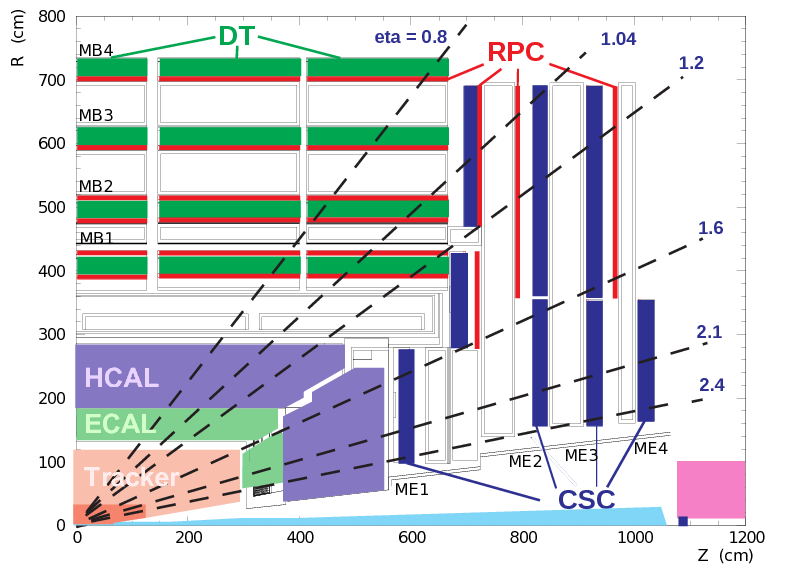
\includegraphics[width=0.6\textwidth]{./Figures/detector/muon_sys}
  \caption{A quarter cross section of the CMS muon system showing the DTs in the barrel region ($|\eta| < 1.2$) and the CSCs in the endcap
  region $ 1.2 < |\eta| < 2.4$. RPCs are layered with the DTs and CSCs in the range $|\eta| < 1.6$ to provide an independent but complementary measurement~\cite{CMS}.}
  \label{fig:MUON_SLICE}
\end{figure}

The performance of the muon system has been measured using early 7 \TeV~beam and cosmic muon data~\cite{muon_performance}. 
The efficiency of muon reconstruction is typically 96 -- 99\%. The muon system relies on the effective
absorption of charged particles other than muons in the layers of the detectors.
`Punch through' of such particles is reduced to $\sim 5\%$ for the first muon station and to
$\sim 0.2\%$ for further stations. The momentum resolution 
was measured as $\sim 1.8\%$ ($10\%$) for muons of $\pt=20\GeV$ ($\pt=1000\GeV$) 
using 7 \TeV~beam and cosmic muon data. 

\section{Data acquisition system}

Data acquisition (DAQ) is a major challenge for the CMS experiment as the collision rate far exceeds reasonable processing 
and storage capabilities that would be required if all data were to be fully reconstructed. It is critical
for the CMS physics programme that 
possible signal events are selected swiftly and efficiently while keeping to constraints placed on data bandwidth, storage and 
latency. The LHC produces bunch crossings at a rate of up to 40MHz but can only
store $\sim1$kHz for offline analysis~\cite{daq_tdr}. The required rejection power of $10^4$ is too large to be achieved
in a single processing step while maintaining a high efficiency and so the task is split into two stages.
The first step, Level-1 trigger (L1 trigger), is a hardware system that uses a small subset of the event information
to accept or reject events. The L1 trigger reduces the rate of events which must be completely 
read from the detector buffers to a maximum of 100kHz. Even with this reduction, 100 Gbytes/s must be transferred to the surface
to be processed by the second step, the High Level Trigger (HLT), which reduces the rate to a peak of $\sim1$ kHz which is 
read to tape to be fully reconstructed. A schematic diagram of the DAQ process is show in Fig~\ref{fig:DAQ_SLICE}. 
The selections at both the L1 trigger and HLT steps are designed to optimise efficiency given the constraints 
of acceptable rate and latency.

\begin{figure}
\centering
    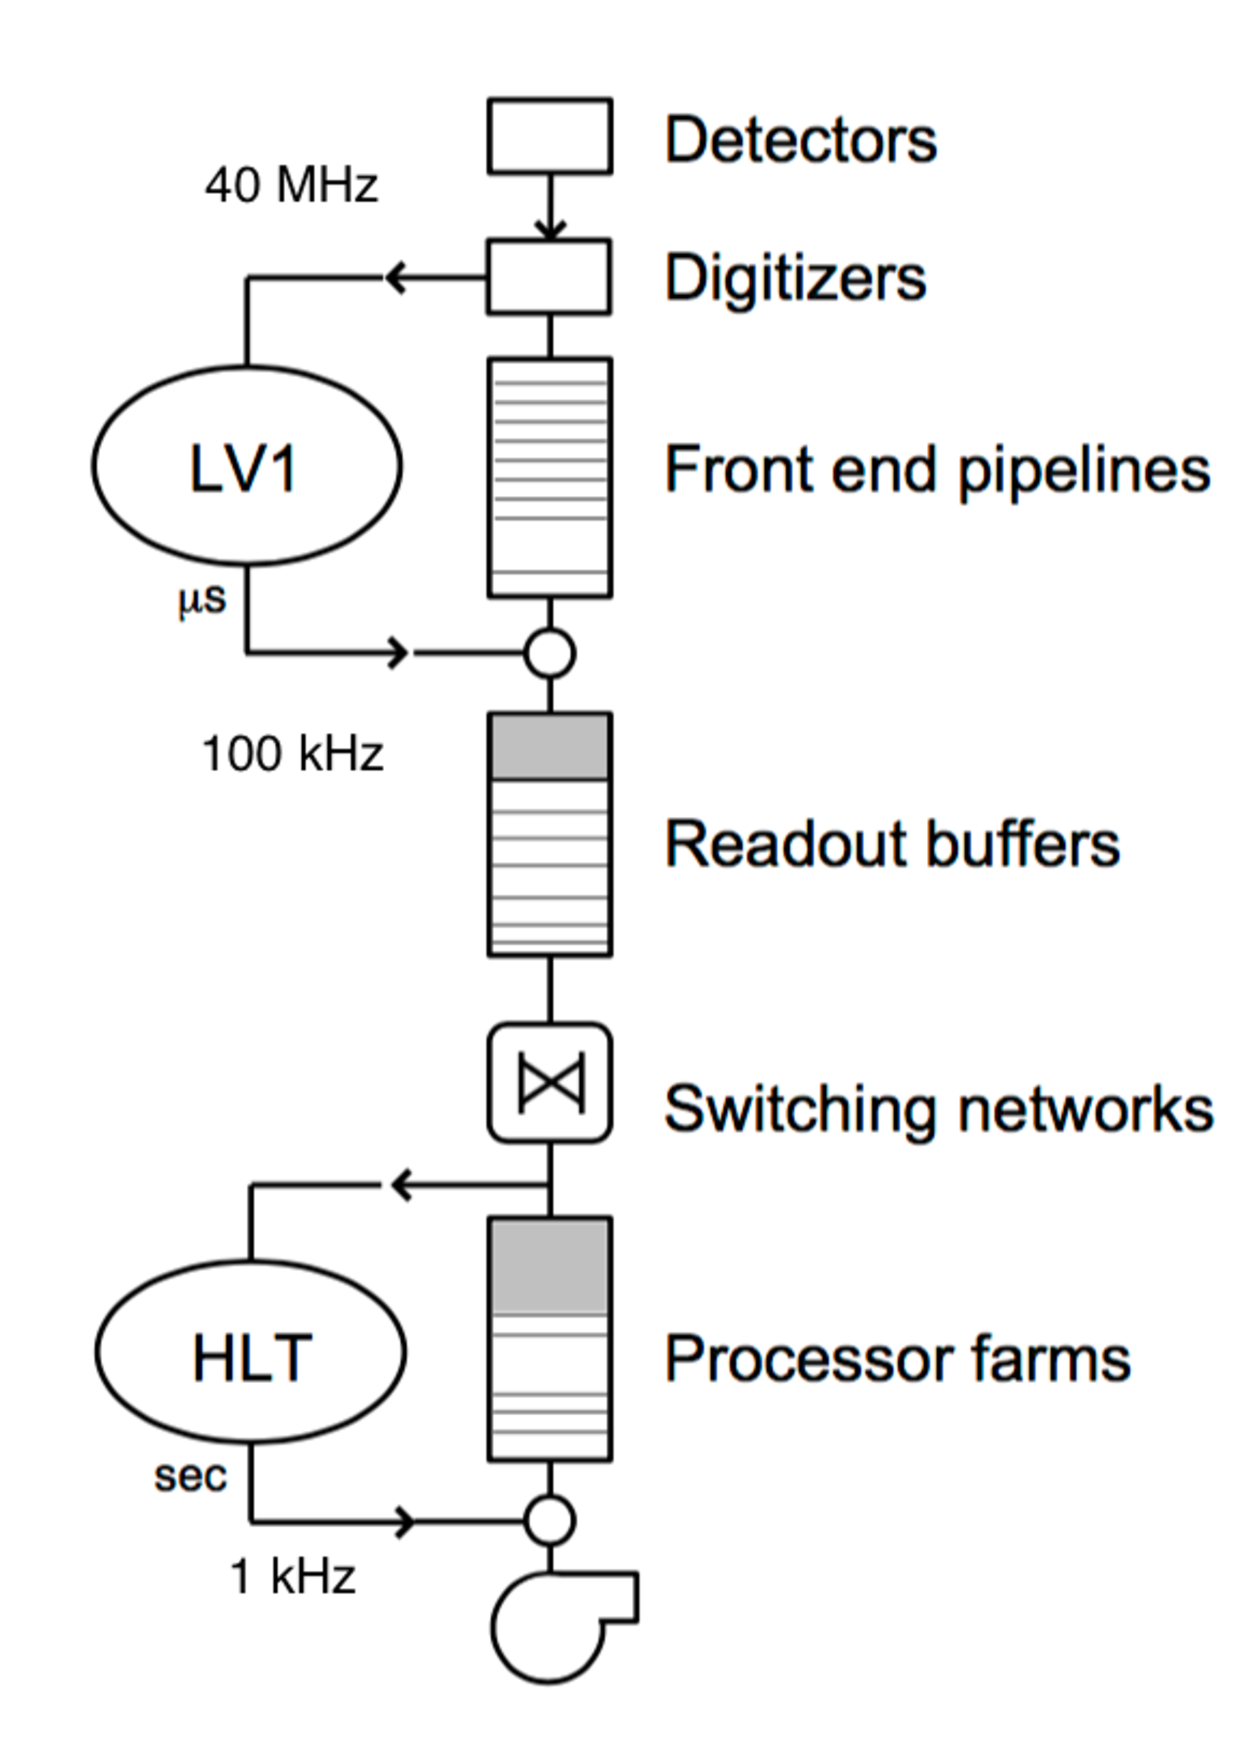
\includegraphics[width=0.6\textwidth]{./Figures/detector/daq_sys}
  \caption{Diagram of the CMS DAQ system showing the data flow from the detector through the L1 trigger
and the HLT. The approximate rate into each system as well as the maximum time for a decision are indicated~\cite{daq_tdr}.}
  \label{fig:DAQ_SLICE}
\end{figure}

\subsection{Level-1 trigger}

The L1 trigger system is the first step in selection for all data collected by the CMS detector. The event selection 
is timed using a local clock synchronised to the LHC bunch collision which initiates the partial readout and processing of 
detector subsystems and storage of data in the L1 trigger pipelines. The limited pipeline depth restricts the latency for L1 trigger decision to a budget of $3.2\mu s$,
of which $\sim2\mu s$ must be used for transmission of data~\cite{daq_performance}. This necessitates the use of fast, high performance electronics
and optical links to rapidly reconstruct the event and make the trigger decision. The timing restriction allows only 
a partial reconstruction using a reduced information set from the calorimetry and muon subsystems only. Dedicated electronics
reconstruct physics objects in local regions of the detector that are passed to the global trigger, which constructs global
quantities and makes the final trigger decision. The various requirements are known as trigger seeds. 
If accepted, the event is fully read and transmitted to the final triggering
stage. The L1 trigger has undergone two stages of upgrade for the start of Run 2, described in detail in Chapter~\ref{cha:triggerUpgrade}.

\subsection{High Level Trigger}

The HLT receives the full detector information read from the CMS detector. It is able to use this to perform 
a full reconstruction with all detector subsystems, allowing a performance similar to the offline reconstruction. However, 
though the maximum processing time per event is significantly greater than for the L1 trigger, latency constraints 
require the use of simplified reconstruction algorithms. The reconstruction is performed using modular trigger paths
that each sequentially execute reconstruction and selection criteria~\cite{daq_performance}. 

Events which pass the HLT selection are transmitted to the CERN `Tier-0' for permanent storage and reconstruction. 
The GRID computing infrastructure allows the offline reconstruction and processing to be distributed to dedicated 
computing sites across the globe~\cite{grid_tdr}. Overall, despite these efforts to reduce data rate, 
several peta-bytes of data must still be recorded every year for offline analysis, in addition to 
a similar quantity of simulated events.

\section{Simulation}

To confront data from experimental observations with a theoretical hypothesis requires an accurate
simulation of both background and signal processes and of their interactions with the CMS detector.
This is extremely challenging at the LHC due to the wide range of particle multiplicities and momenta 
from the p-p collisions, often in non-perturbative regimes. The simulation of events at CMS 
is factorised into five stages: the hard scattering, fragmentation, hadronisation, decay and 
detector simulation. A generic review of simulation for particle physics can be found in~\cite{sim_rev}.

The hard scattering models the interaction between the two collision partons. The energy carried by each
is sampled from the parton density function depending on the hard-scatter energy scale~\cite{pdf}. 
This process is simulated using the \PYTHIA and \MADGRAPH generators~\cite{PYTHIA,MADGRAPH}. 

The fragmentation and hadronisation is performed using dedicated showering and hadronisation algorithms with
generators such as \PYTHIA or \HERWIG~\cite{PYTHIA,HERWIG}. The fragmentation is an iterative process of repeated 
radiation of soft gluons and quarks performed until the calculation becomes non-perturbative. 
The particles are then clustered into colourless bound state with different techniques used
to connect the colour flow from initial partons to the final state partons, depending on the generator. 
Unstable particles formed at this stage then undergo further decay. Subsequent $\tau$ lepton 
decay is simulated using the dedicated \TAUOLA~generator~\cite{TAUOLA}. The particles formed 
during this stage are referred to as generator level particles. 

The simulated background samples are normalised using cross sections calculated with PROSPINO~\cite{Prospino}
to next-to-leading order (NLO) and next-to-next-to-leading order (NNLO) in $\alpha_s$.

The effects of pileup are simulated by combining the generated output with a minimum bias sample 
with a mean of twenty simultaneous interactions. This is done in a 12 bunch 
crossing window of the signal event to include the effects of both 
out-of-time and in-time pileup.

The interactions with the CMS detector of the generated particles must be simulated. For the background processes
a full detector simulation is performed using \GEANTfour~\cite{GEANT}, while for the simulated
samples the detector response is simulated using the CMS fast simulation package~\cite{fastsim}.
% This can then be used as the inputs for the reconstruction stages described 
% in Chapter~\ref{cha:reco}.

